% Chapter Template

\chapter{Related Work} % Main chapter title

\label{Chapter:RelatedWork}

%\subsubsection*{\color{mygray}[Chapter under work]}

%----------------------------------------------------------------------------------------
%	SECTION 1
%----------------------------------------------------------------------------------------

\section{Role of rheological properties in near field electrospun fibers morphology \cite{Flores2017}}

Flores studied SU-8 2002 polymer solutions in cyclopentanone with poly(ethylene) oxide (PEO) and tetrabutylammonium tetrafluoroborate (TBATFB). For that purpose, several samples were prepared with the adequate amounts of PEO and TBATFB with 5 $m l$ of SU-8 2002 and stirred at 160 $r p m$ for one hour at 75 $^\circ C$ in the absence of light. A 5 $m l$ syringe was used to extract the solution from the preparation vial. Finally the syringe was placed upside down for 24 hours to get rid of any bubbles within the solution. Table \ref{tbl:FloresSamples} lists the set of samples that were prepared as values in $w t \%$, dissolved in SU-8 2002.

\begin{table}[th]
\caption{Set of prepared samples}
\begin{center}
\begin{tabular}{ c c c c c c c } 
\hline
\text{} & \multicolumn{2}{c}{Serie A} & \multicolumn{2}{c}{Serie B} & \multicolumn{2}{c}{Serie C} \\
\hline
Sample & PEO & TBATFB & PEO & TBATFB & PEO & TBATFB \\
\hline
1 & 0.00 & 0.00 & 0.00 & 0.50 & 0.50 & 0.00 \\
2 & 0.25 & 0.25 & 0.25 & 0.50 & 0.50 & 0.25 \\
3 & 0.50 & 0.50 & 0.50 & 0.50 & 0.50 & 0.50 \\
4 & 0.75 & 0.75 & 0.75 & 0.50 & 0.50 & 0.75 \\
5 & 1.00 & 1.00 & 1.00 & 0.50 & 0.50 & 1.00 \\
\hline
\label{tbl:FloresSamples}
\end{tabular}
\end{center}
\end{table}

All the samples were executed in a rheometer (Physica MCR 301, Anton Paar) with a cone-and-plane geometry of diameter 24.979 $m m$, angle 4.014$^\circ$ and truncation of 249 $\mu m$. The measurements were performed at a temperature of 25 $\pm$ 0.1 $^\circ C$. For amplitude sweep measurements, the angular frequency was settled at 10 $s^{-1}$, and the percentage amplitude gamma $\% \gamma$, was varied from 0.1 to 1000\%. In flow curve tests, shear rate was applied from 0.1 to 100 $s^{-1}$. For frequency sweeps, the percentage of amplitude gamma, $\% \gamma$, was varied from 0.1 to 100 $s^{-1}$. During the measurements, the rheometer sample area was saturated with cyclopentanone to avoid solvent evaporation.

\subsection{Rheological Characterization : \textbf{Amplitude Sweep}}
The "Serie A`` result measurements indicate that the storage modulus $G'$ is smaller than the loss modulus $G''$. Both moduli have a parabolic behaviour. At low deformation the values of the moduli increase until they become stable at between 1 and 10 $\% \gamma$. After the stabilization, both modulus start to decrease. The increase of PEO and TBATFB concentration $G'$ and $G''$ also increase. Figure \ref{fig:SerieAampSweep} shows the amplitude sweep for the samples of "Serie A``.

\begin{figure}[th]
\centering
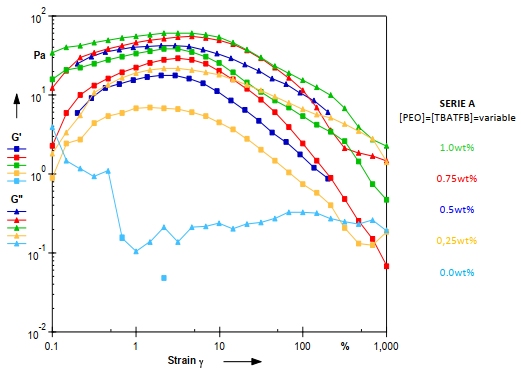
\includegraphics[width=0.75\textwidth]{./Figures/SerieAampSweep.png}
\decoRule
\caption[Serie A - Amplitude Sweep]{Serie A - Amplitude Sweep}
\label{fig:SerieAampSweep}
\end{figure}

The results within Figure \ref{fig:SerieAampSweep} showed that no clear linear viscoelastic region is present. The material has influenced by small deformations, hence it is very sensitive to external forces. No yield point was encountered as the moduli separate from each other with the increase of deformation.

Figure \ref{fig:SerieBampSweep} illustrates the results obtained from the amplitude sweeps of Serie B samples. As shown in the figure, the concentration of 0 $w t \%$ shows a constant viscous modulus at 0.2 $Pa$. the 0.25 $w t \%$ concentration sample presented a similar behaviour to the 0 $w t \%$ sample but with a constant value of $G'$ at 2 $Pa$. The other concentrations show a similar parabolic behaviour as the ones in Serie A.

\begin{figure}[th]
\centering
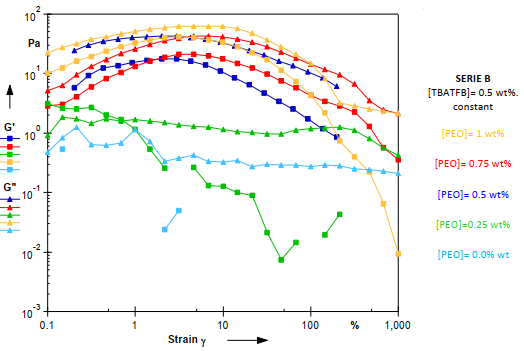
\includegraphics[width=0.75\textwidth]{./Figures/SerieBampSweep.png}
\decoRule
\caption[Serie B - Amplitude Sweep]{Serie B - Amplitude Sweep}
\label{fig:SerieBampSweep}
\end{figure}

\begin{figure}[th]
\centering
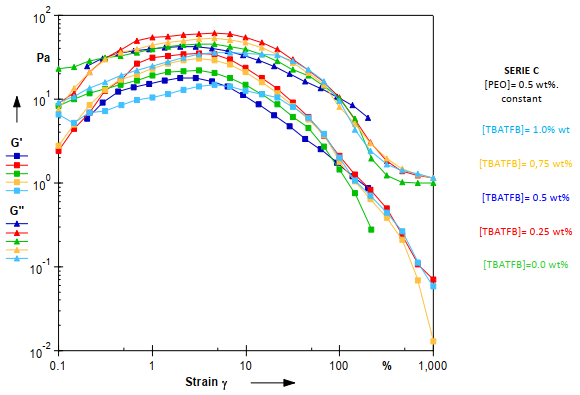
\includegraphics[width=0.75\textwidth]{./Figures/SerieCampSweep.png}
\decoRule
\caption[Serie C - Amplitude Sweep]{Serie C - Amplitude Sweep}
\label{fig:SerieCampSweep}
\end{figure}

The amplitude sweep results of Serie C are depicted in Figure \ref{fig:SerieCampSweep}. Similar to series A and B, results show that the storage modulus $G'$ is smaller than the loss modulus $G''$ with a parabolic behaviour. Typically, the amplitude sweep is to determine the amplitude to be used in frequency sweeps. The amplitude determined by the amplitude sweeps shall keep the material structure undisturbed is known as the linear viscoelastic region (LVER). However, no LVER was found in the samples. For that reason, the percentage of amplitude gamma $\% \gamma$ was found by trial and error. Flores discovered that a $\% \gamma = 20$ has the best performance. 

\subsection{Rheological Characterization : \textbf{Flow Curve}}
Figure \ref{fig:SerieAflowCurve} shows evidence that the equal increase of PEO and TBATFB concentrations result in an increase of shear viscosity rate $\gamma$. For concentrations from 1.00 to 0.25 $w t \%$, a slight increase of flow curve strain $\eta$ for low shear rates to 0.3 $s^{-1}$. For shear rates greater than 0.3 $s^{-1}$, the $\eta$ starts to decrease, as the polymer entanglements start to break apart, reducing friction between the polymer threads and therefore the viscosity also is reduced. The solution samples show a Newtonian-like behaviour and that may be caused by the use of the solvent cyclopentanone and by the small sized SU-8 2002 molecules.

\begin{figure}[th]
\centering
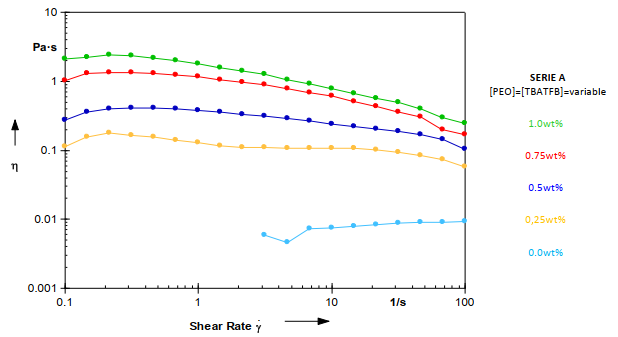
\includegraphics[width=0.75\textwidth]{./Figures/SerieAflowCurve.png}
\decoRule
\caption[Serie A - Flow curve]{Serie A - Flow curve}
\label{fig:SerieAflowCurve}
\end{figure}

From the results in Figure \ref{fig:SerieAflowCurve}, it is noticeable that the addition of small amounts of PEO and TBATFB cause a change of one order of magnitude in shear viscosity in small concentrations and a triple change in high concentrations.

Series B flow curve results (Figure \ref{fig:SerieBflowCurve}) do not show a clear correlation between PEO concentrations and shear viscosity. For PEO of 1 $w t \%$, a slow increase in $\eta$ is present with the increase of shear rate, after $\gamma$ drops from 2 to 0.8 $Pa s$, a shear thinning behaviour is present. For 0.50 and 0.75 $w t \%$ concentrations, a shear thinning behaviour is present throughout the plot. For the 0.50 $w t \%$ sample, viscosity value varied between 0.2 and 0.4 $Pa s$; and between 0.5 and 2.0 $Pa s$ for the 0.75 $w t \%$ sample. Viscosity is stabilized at 0.1 $Pa s$ when the shear rate is between 1 and 20 \% for the sample of PEO $w t \%$. After stabilization, the viscosity decreases from 0.1 to 0.02 $Pa s$ for shear rates between 20 to 100 $s^{-1}$. For PEO 0.00 $w t \%$, a high variation is present in viscosity readings due to the presence of electrolytes cause amendments in the polymer chain within the solution.

\begin{figure}[th]
\centering
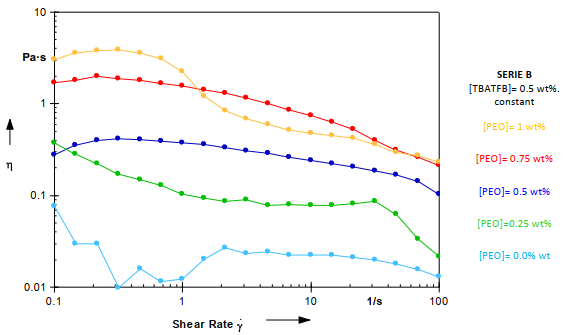
\includegraphics[width=0.75\textwidth]{./Figures/SerieBflowCurve.png}
\decoRule
\caption[Serie B - Flow curve]{Serie B - Flow curve}
\label{fig:SerieBflowCurve}
\end{figure}

The flow curve results of Serie C are presented in Figure \ref{fig:SerieCflowCurve}. The sample with 1 $w t \%$ TBATFB concentration shows a shear thinning behaviour for shear rates varying between 0.1 to 15 $s^{-1}$. The 1 $w t \%$ sample describes a drop in viscosity for shear rates between 15 to 20 $s^{-1}$ followed by a stable state. A similar behaviour is observed for a concentration of 0.75 $w t \%$. and less evident for 0.0 $w t \%$. For concentrations of 0.5 $w t \%$ and 0.25 $w t \%$ the behaviour of the shear viscosity is similar.

\begin{figure}[th]
\centering
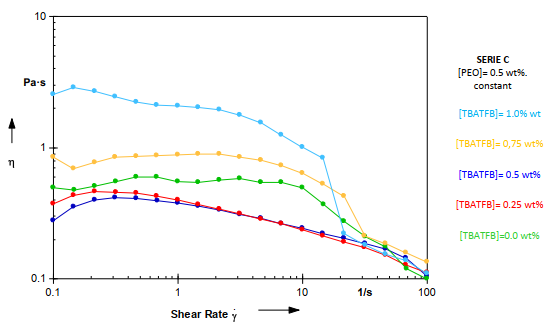
\includegraphics[width=0.75\textwidth]{./Figures/SerieCflowCurve.png}
\decoRule
\caption[Serie C - Flow curve]{Serie C - Flow curve}
\label{fig:SerieCflowCurve}
\end{figure}

\subsection{Rheological Characterization : \textbf{Frequency Sweep}}
Figure \ref{fig:SerieAfreqSweep} shows that the solution with the lowest concentration of PEO and TBATFB has a decreasing behaviour of the viscosity, but for values greater to 3 $s^{-1}$ in frequency, the viscosity starts to increase. The solutions from 0.25 $w t \%$ to 1.00 $w t \%$ have the same shear-thinning behaviour. A direct relation between the concentrations and the viscosity values is discovered, where a small drop of viscosity is presented with the decrease of additive concentration.

\begin{figure}[th]
\centering
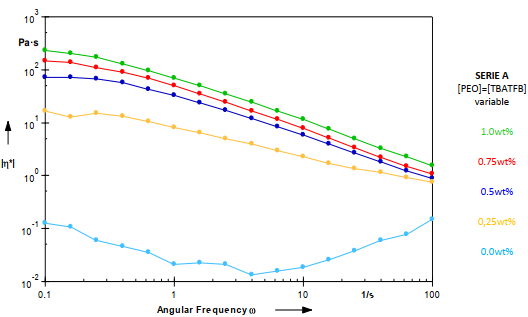
\includegraphics[width=0.75\textwidth]{./Figures/SerieAfreqSweep.png}
\decoRule
\caption[Serie A - Frequency Sweep]{Serie A - Frequency Sweep}
\label{fig:SerieAfreqSweep}
\end{figure}

Figure \ref{fig:SerieBfreqSweep} shows the frequency sweep results from Serie B. The presented behaviour is similar to Serie A. for the lower concentrations of PEO, the equipment has not enough sensibility to make measurements of the storage modulus because this one is very low. At PEO 0.25 $w t \%$, the viscosity remains almost constant at 1 $Pa s$, but as in Serie A a little variation of viscosity is presented at the lowest values of angular frequency. On the other hand, for the 0.5, 0.75 and 1.00 $w t \%$ concentrations, the viscosity is similar. At 100 $s^{-1}$, the three high concentration samples converge to 2 $Pa s$. It is imperative to assume that 0.5 $w t \%$ is the critical concentration, under this concentration the systems present different behaviours since the molecules have enough room to diffuse and break entanglements. When the critical entanglement concentration is exceeded, the polymer threads overlap and become tangled, therefore no more entanglements are no longer possible.

\begin{figure}[th]
\centering
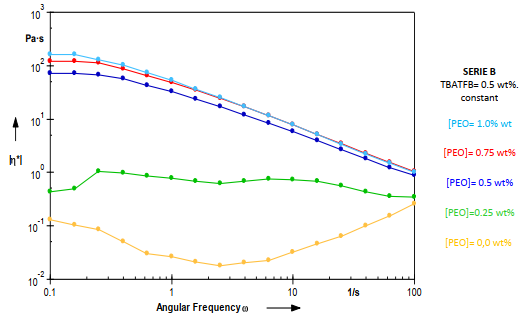
\includegraphics[width=0.75\textwidth]{./Figures/SerieBfreqSweep.png}
\decoRule
\caption[Serie B - Frequency Sweep]{Serie B - Frequency Sweep}
\label{fig:SerieBfreqSweep}
\end{figure}

The frequency sweep behaviours of Serie C are presented in Figure \ref{fig:SerieCfreqSweep}. The figure does not indicate a clear correlation between the viscosity and the addition of TBATFB. All samples have a similar behaviour and magnitude, except for the 0.75 $w t \%$ TBATFB concentration sample as it presents a non uniform behaviour. At low frequencies, the viscosity increases, then it remains constant at 20 $Pa s$ until a frequency value of 4 $s^{-1}$; the viscosity drastically decreases to 1 $Pa s$ and remains constant at that value. The 1.00 $w t \%$ sample has a decreasing viscosity behaviour at higher angular frequencies. 

\begin{figure}[th]
\centering
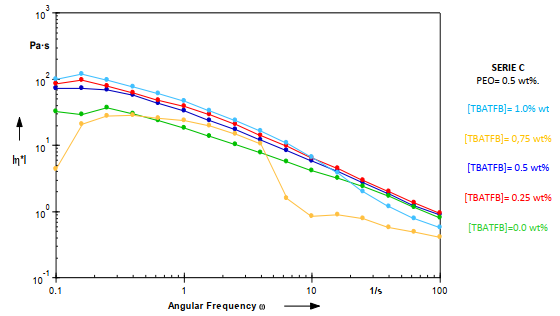
\includegraphics[width=0.75\textwidth]{./Figures/SerieCfreqSweep.png}
\decoRule
\caption[Serie C - Frequency Sweep]{Serie C - Frequency Sweep}
\label{fig:SerieCfreqSweep}
\end{figure}

Flores work \cite{Flores2017} carried out a series of experiments in order to correlate the rheological properties of polymer solutions used in electro-mechanical spinning processes for the fabrication of carbon micro structures. Shear flow and dynamic measurements tests such as flow curves, amplitude sweeps and frequency sweeps were carried in an oscillatory rheometer to study the rheological behaviour of polymeric solutions of SU-8 2002, an epoxy-based negative photoresist, Poly(ethylene) oxide (PEO), a flexible, non-ionic polymer, and TBATFB (Tetrabutylammonium tetrafluoroborate) that acts as an electrolyte.

The concentrations of additives were varied from 0 $w t \%$ to 1.0 $w t \%$ with increments of 0.25. To observe the effects of each additive it was proposed a set of concentrations where both additives were equally varied (Serie A), TBATFB was constant the only PEO variations (Serie B), and PEO constant concentration with TBATFB variations (Serie C). It was found that the variation of the additives (PEO and TBATFB) affects the
rheological behavior of the solution. Typically, the addition of PEO increase the
elongational and shear viscosities while the addition of TBATFB modifies this property
but in a non-predictable manner. The solutions do not present yield stress as can be
seen in Amplitude Sweep and Frequency Sweep measurements.

\clearpage

\section{Advanced Manufacturing Techniques for the Fabrication and Surface Modification of Carbon Nanowires \cite{Cardenas2017}}

As stated by Cardenas \cite{Cardenas2017}, the following parameters play an important role in the graphitic content on the fabrication of carbon nano-wires through electrospinning:

\begin{enumerate}
\item The thickness of the produced polymeric wires,
\item the chemical composition and viscoelasticity of the polymeric solution,
\item the molecular alignment of the polymer,
\item the heat treatment temperature,
\item the mechanical pulling on the polymer jet during electrospinning,
\item the alignment of polymer chains induced by the presence of an electric field, and
\item the catalysts and solvents within the polymer solution.
\end{enumerate}

Cardenas reviewed different polymer fabrication techniques and materials to produce carbon nano-wires. Within Cardenas' work the following parameters were evaluated to study the desirable characteristics for building highly sensitive sensor devices: a) the chemical composition and viscoelasticity of the polymer solution, b) the thickness of the produced polymeric wires, c) the mechanical pulling on the polymeric jet during electrospinning, and d) the alignment of the polymer chains induced by the presence of an electric field. Cardenas' work states that various methods are implemented to produce nanofibers, such as laser ablation, chemical vapor deposition, discharge, and vapor growth. However, those techniques are abandoned due to their low yield output and expensive equipment. Whereas electrospinning (ES) of polymer solutions is a promising technique for simple and inexpensive fabrication of carbon nano-wires, which can be combined with a moving collector to yield even thinner fibers.

The production of carbon structures involves to main procedures: a) polymer patterning such as photolithography, electrospinning, Computer Numerical Control (CNC), molding, hot embossing, and recently, Multiple Photon Polymerization; and b) carbonization, which induces further thinning of the patterned polymer and its conversion into carbon. Cardenas conducted some experiments to characterize and analyze carbon nano-wires. Polymeric SU-8 nano fibers were produced by two different methods; for each method different polymer solutions were employed.

\subsection{Method 1 : }

\subsubsection{Polymer Solution}
The polymeric solution was composed by 2 $ml$ of SU-8 2002 mixed with 0.5 $w t \%$ of PEO and 0.5 $w t \%$ of TBATFB to increase its conductivity and yield soother polymer jets during electrospinning. Magnetic stirring was performed for 1 $hr$ at 75 \textdegree{}$C$ with $rpm$ values between 100 and 150.

\subsubsection{Deposition}
A voltage around 100 $V$ was applied between a dispensing needle and the collector stage. The needle to collector distance was set to 100 $\mu m$. The collector was attached to a mechanically motorized stage, which allowed the SU-8 nanofibers patterning into the SU-8 microstructures. Three different stage velocities were tested (20,40 and 60 $mm/s$) to study the influence on the wire geometry. Acceleration of the stage was set to 500 $mm/s^{2}$. After deposition, samples were exposed to UV light for 45 $min$ to complete cross-linking.

\subsection{Method 2 : }

\subsubsection{Polymer Solution}
The solution was composed of 4 $ml$ of SU-8 2025, 4 $mg$ of TBATFB and 80 $\mu L$ of SU-8 thinner. The solution was stirred for 1.5 $hrs$ at 100 $rpm$ at 75 \textdegree{}$C$.

\subsubsection{Deposition}
To pattern the fiber exactly on top of the SU-8 electrodes, a routine was set to move the needle relative to the collector. The polymer solution was dispensed at a rate of 8.847 $nL / min$ using a programmable syringe pump. A voltage of 200 $V$ was applied between the collector plate and the needle tip, and the polymer solution was allowed to flow for between 15 to 30 $min$ until it was stable. A higher voltage had to be applied compared to Method 1 due to the higher viscosity of the SU-8 2025 solution. Once a steady flow was achieved, the collector was moved relative to the needle tip using the motorized stage. The mechanical parameters used during were: a) velocity of 5000 $\mu m/s$, an acceleration of 2500 $\mu m/s^{2}$. The sample was exposed to UV light for 45 min to ensure complete cross-linking of the deposited SU-8 nanofiber.

\subsection{Results and Discussion}
To test the possibility of using SU-8 to fabricate carbon nano-wires, samples were pyrolyzed in an inert environment. Samples prepared by Method 1 failed the pyrolyzation as the deposited wires were mostly liquid before carbonization. The fibers produced by Method 2 had a yield rate of 81 $\%$. The diameters after pyrolysis were analyzed and measured using SEM micrographs.

Cardenas \cite{Cardenas2017} states that the geometry of the carbon nano-wires is also an important characteristic that affects the carbon structure conductivity, mechanical and thermal characteristics and crystallinity. The conducted experiments showed some techniques and materials that have been applied to fabricate carbon nano-wires, as well as the effects that fabrication parameters have on the final geometry of the carbon structures. The newly technique of electro-mechano-spinning (EMS) involved new polymer solutions along with a systematic deposition process. Cardenas found that the EMS proposed manufacturing technique yielded normally distributed diameters of 204 $nm$ with low variability, which is significantly reduced the uncertainty in the fabrication of carbon nano-wires.

\clearpage

\section{FIND PAPER THAT CONFIRMS THAT WITH THE INCREASE OF PEO CONCENTRATION, THE POROSITY DENSITY INCREASES IN CARBON STRUCTURES AFTER PYROLYSIS. \cite{newPAPER}}

As explained in Section \ref{sec:pyrolysis}, the pyrolysis process is implemented to thermally decompose organic material into carbon. ...

%-----------------------------------
%	SUBSECTION 1
%-----------------------------------


